\chapter{Airfoil}\label{cp:airfoil}

\section{Basic Airfoil Dimensions}

The primary goal at this point in the design process is to maximize time aloft, also known as endurance. To help our aircraft ``glide'' more easily and reduce the thrust required to maintain \acrfull{slf}, we chose to start with a wingspan of \qty{216}{\centi\meter} (\qty{85}{in}), just under the maximum wingspan dictated by the course requirements.

With the wingspan selected, we determined our chord length by assuming an \acrfull{ar} of approximately \num{10}. Then, by using the equation for \acrshort{ar} for a rectangular wing, \autoref{eq:ar},

\begin{align}
    AR &= \frac{b}{c}\label{eq:ar}
\end{align}

\noindent where \acrshort{ar} is the aspect ratio, \gls{b} is the wingspan, and \gls{c} is the wing chord length, we back calculated the chord length to be \qty{20}{\centi\meter} (\qty{8}{in}).

\newpage

\section{Airfoil Selection}

\subsection{Main Wing}

Based on our precursory research, we decided to investigate the suitability of three airfoil shapes, two \acrfull{naca} airfoils and one \acrfull{mh} airfoil, shown in \autoref{fig:airfoil_plots}.

\begin{figure}[htpb]
    \centering
    \begin{subfigure}{0.49\textwidth}
        \centering
        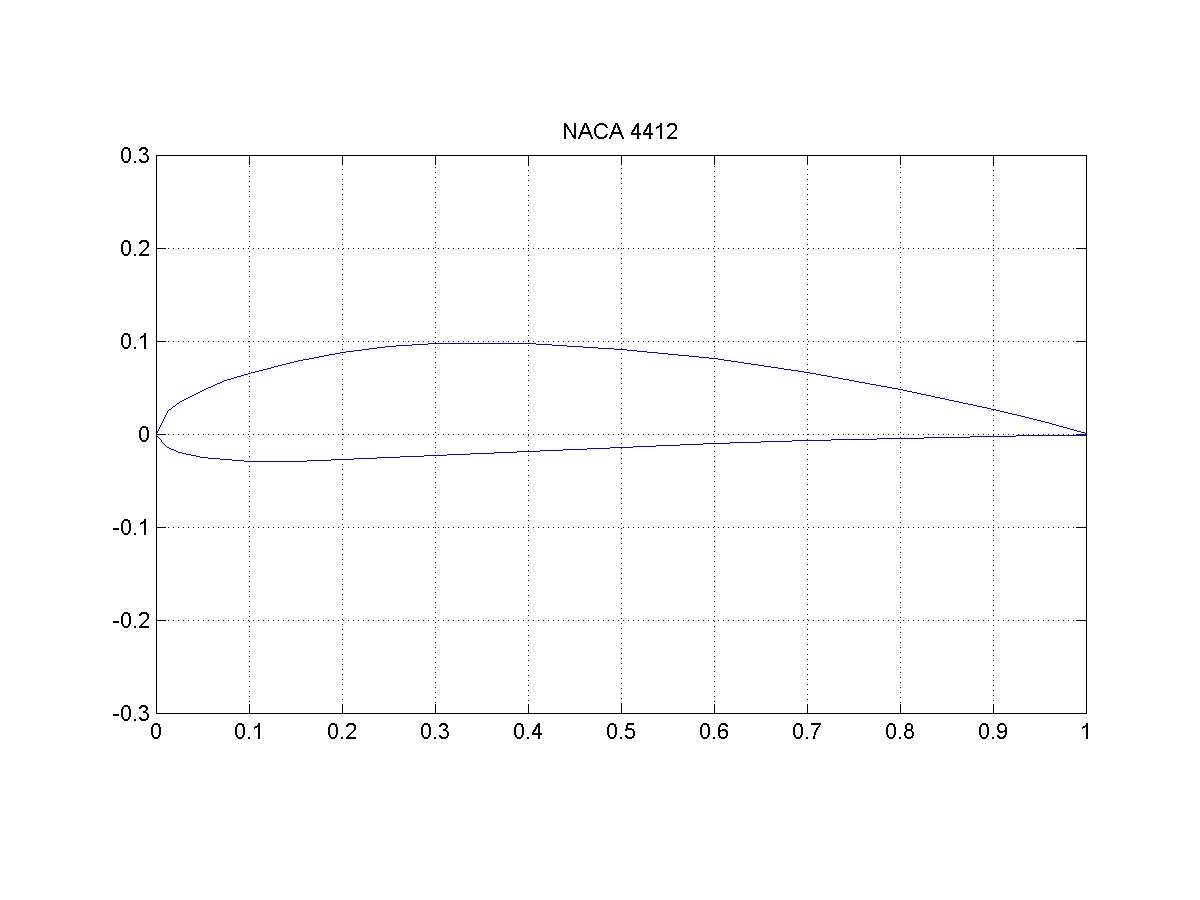
\includegraphics[width=\textwidth]{Figures/NACA_4412.png}
        \caption{Plot of the \acrshort{naca} 4412 airfoil.}
        \label{fig:naca_4412_plot}
    \end{subfigure}
    \begin{subfigure}{0.49\textwidth}
        \centering
        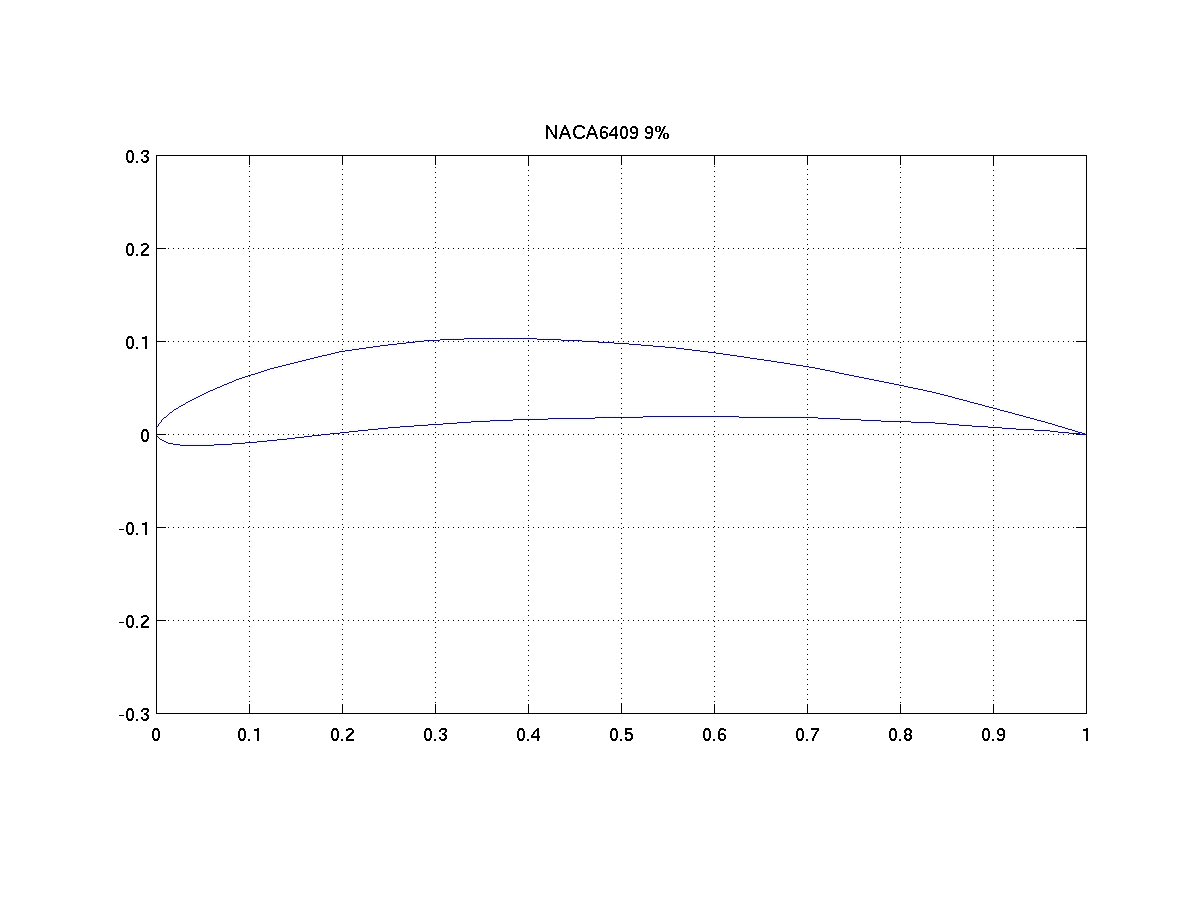
\includegraphics[width=\textwidth]{Figures/NACA_6409.png}
        \caption{Plot of the \acrshort{naca} 6409 airfoil.}
        \label{fig:naca_6409_plot}
    \end{subfigure} \\
    \begin{subfigure}{0.49\textwidth}
        \centering
        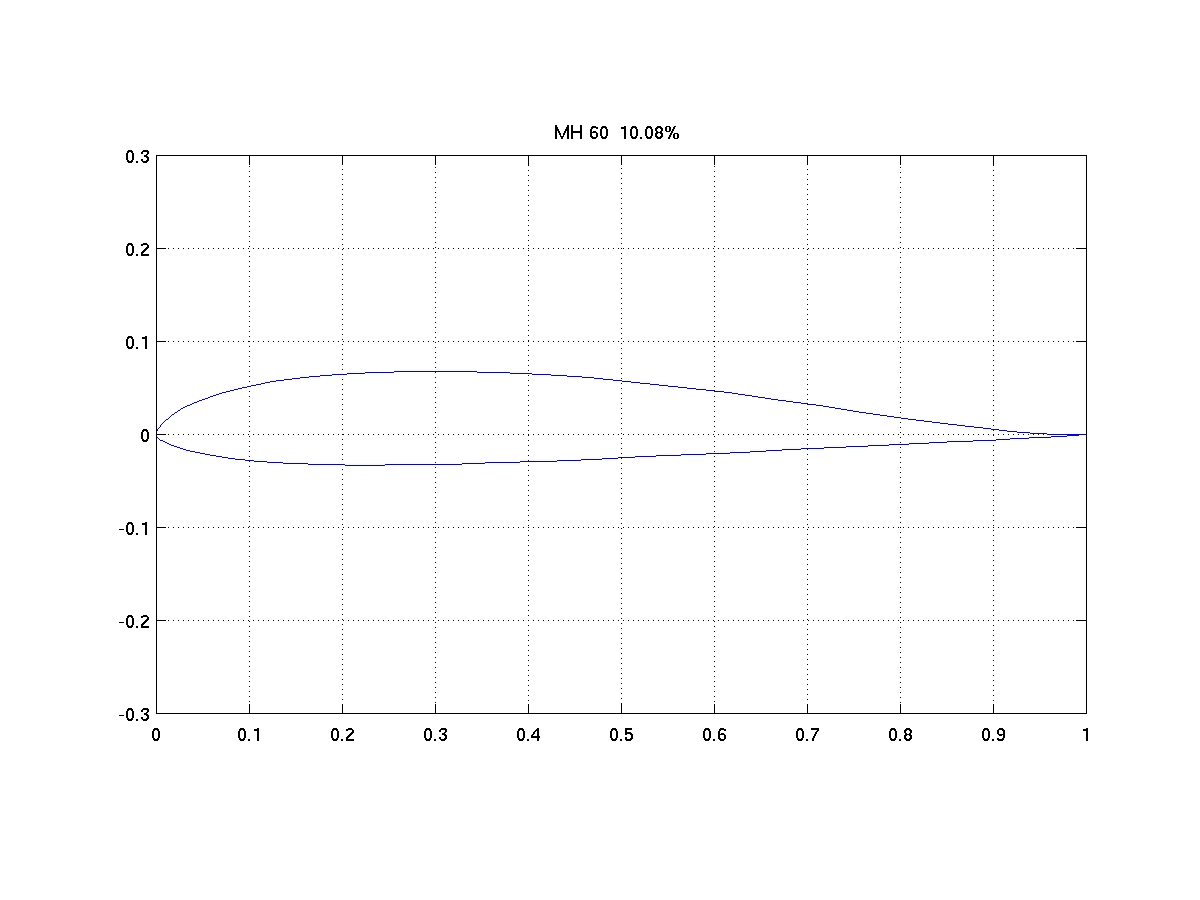
\includegraphics[width=\textwidth]{Figures/MH_60.png}
        \caption{Plot of the \acrshort{mh} 60 airfoil.}
        \label{fig:mh_60_plot}
    \end{subfigure}
    \caption[Airfoil choices for wing]{Plot of each of the airfoils we analyzed for the main wing. Graphs are courtesy of \citet{uiuc2024}.}
    \label{fig:airfoil_plots}
\end{figure}

These airfoils were selected for further analysis because of their historical ability to provide high lift at low speeds. They were also selected for their manufacturing ease, attributed to their simpler shape, in contrast to other high-lift airfoils, which are often very thin and have steep positive camber.

\subsection{Horizontal Stabilizer}

For the horizontal stabilizer, we chose to analyze an \acrfull{e} airfoil, specifically the \acrshort{e}423 (see \autoref{fig:e423_plot}). The \acrshort{e}423 was specifically designed for low-speed aircraft, offering stability and control at slow loitering speeds—crucial for an \acrshort{suas}. It is commonly used in gliders and \acrshort{uav} that require long endurance at low speeds.

\begin{figure}[htpb]
    \centering
    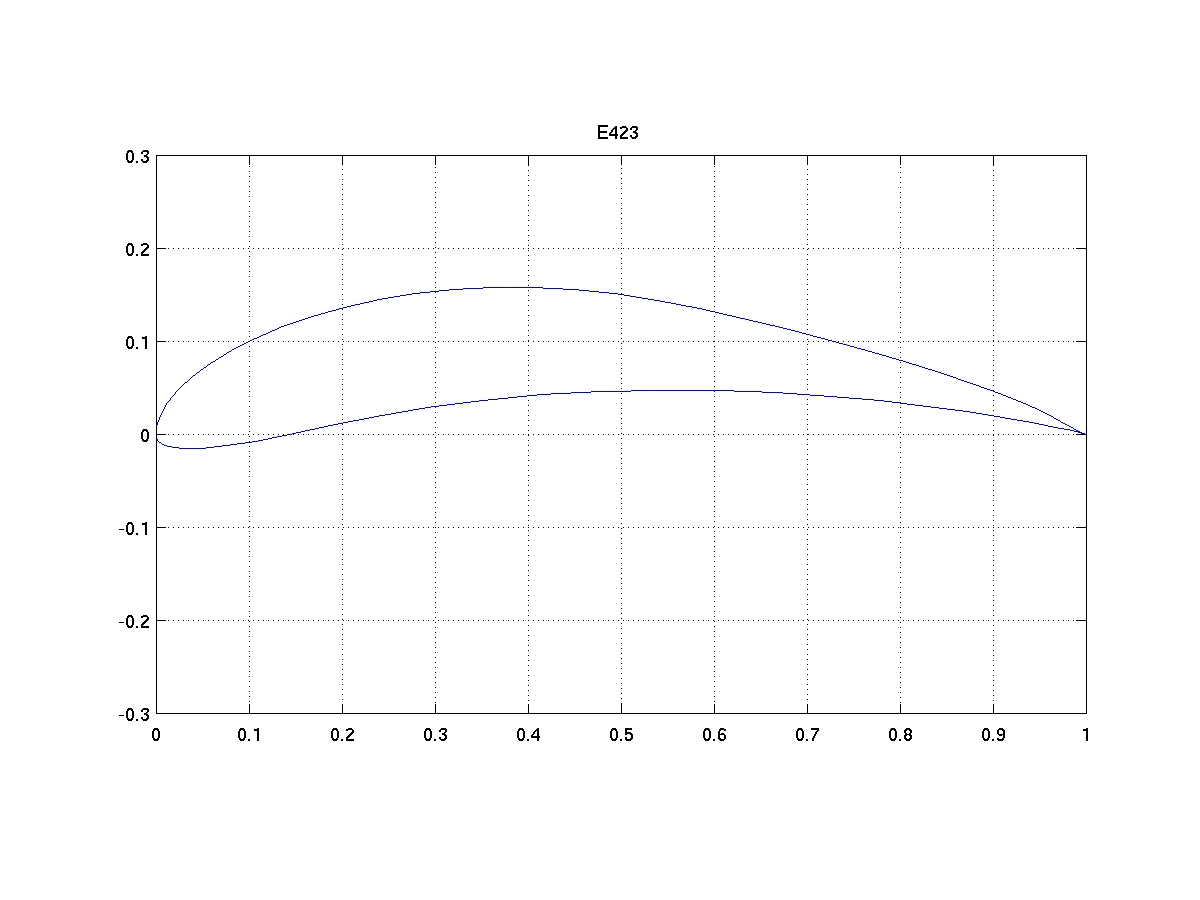
\includegraphics[width=0.49\linewidth]{Figures/E423.png}
    \caption[Airfoil choice for the horizontal stabilizer]{A plot of the \acrshort{e}423 airfoil \citep{uiuc2024}.}
    \label{fig:e423_plot}
\end{figure}

\subsection{Vertical Stabilizer}

Vertical stabilizers are often symmetric airfoils since they have a neutral pitching moment and do not need to generate much lift to create a yawing moment. We chose to analyze the \acrshort{naca}0009 and the \acrshort{naca}0010, shown in \autoref{fig:vertical_stabilizer_airfoil_plots}.

\begin{figure}[htpb]
    \centering
    \begin{subfigure}{0.49\textwidth}
        \centering
        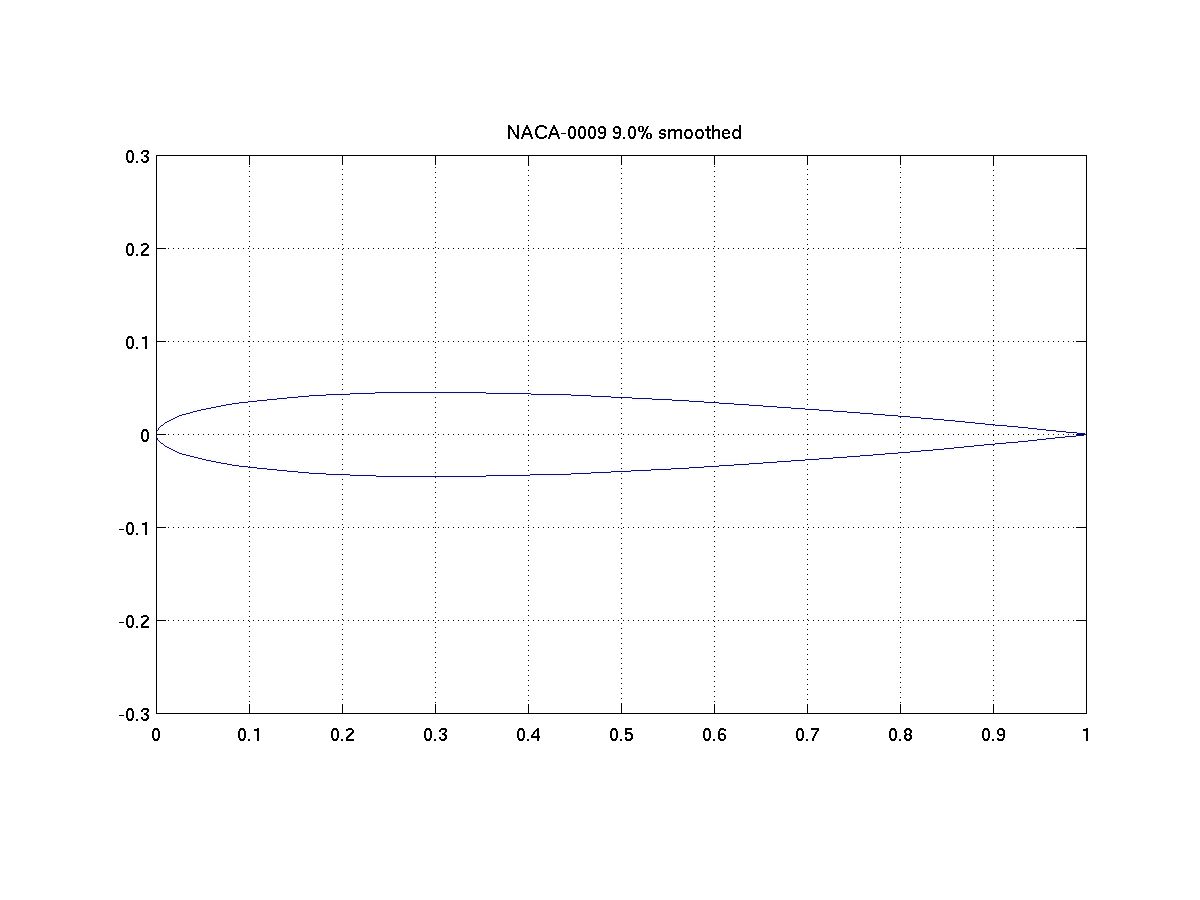
\includegraphics[width=\textwidth]{Figures/NACA_0009.png}
        \caption{Plot of the \acrshort{naca} 0009 airfoil.}
        \label{fig:naca_0009_plot}
    \end{subfigure}
    \begin{subfigure}{0.49\textwidth}
        \centering
        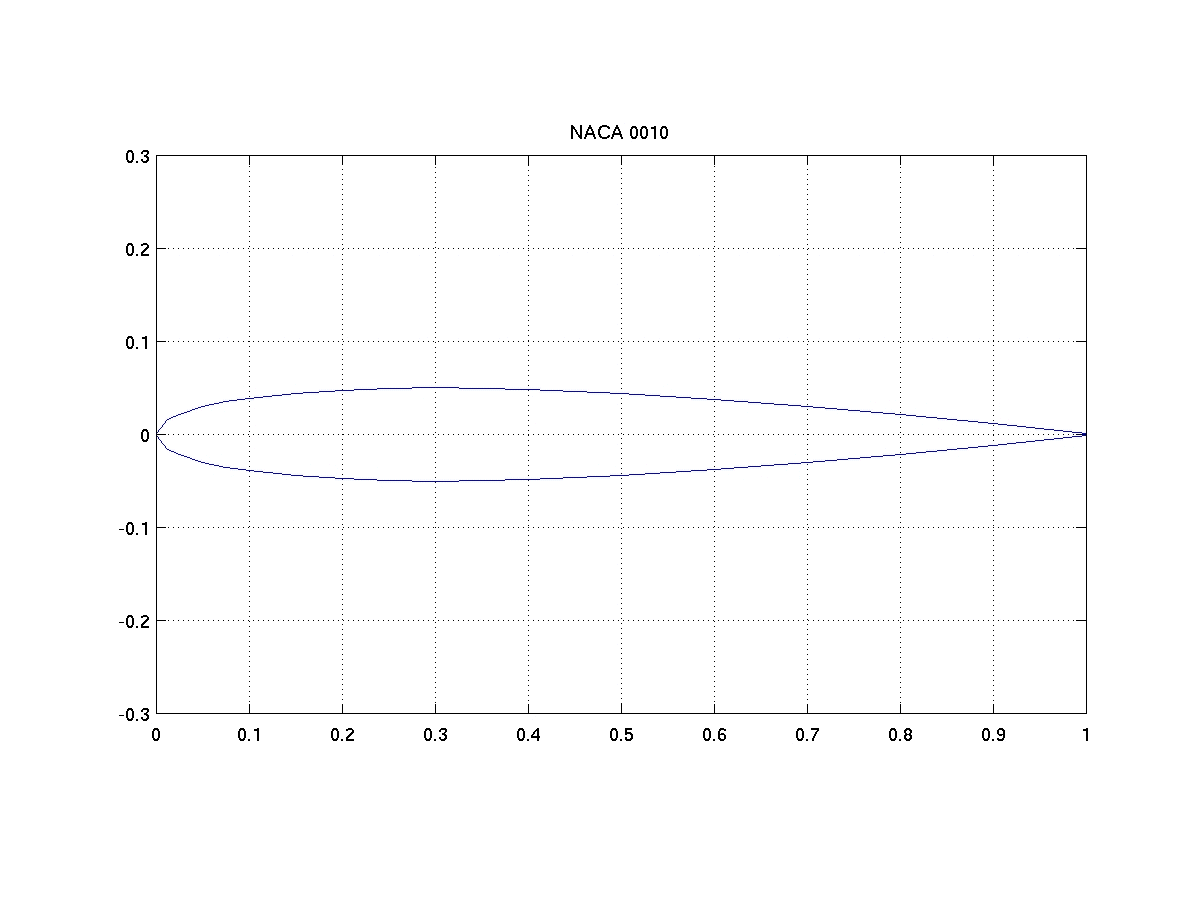
\includegraphics[width=\textwidth]{Figures/NACA_0010.png}
        \caption{Plot of the \acrshort{naca} 0010 airfoil.}
        \label{fig:naca_0010_plot}
    \end{subfigure}
    \caption[Airfoil choices for the vertical stabilizer]{Plot of each of the airfoils we analyzed for the vertical stabilizer. Graphs are courtesy of \citet{uiuc2024}.}
    \label{fig:vertical_stabilizer_airfoil_plots}
\end{figure}

\section{Reynolds Number}\label{sec:reynolds}

To analyze the performance of these airfoils, we had to determine an initial Reynolds number. Since Reynolds number is dependent on atmospheric conditions, we first defined our expected operating conditions. The Banshee needs to loiter above the maximum altitude of \acrfull{cots} \acrshort{suas}, which is typically \qty{120}{\meter} \citep{khan2024}. For the purpose of analysis, we chose a cruise altitude of \qty{150}{\meter} \acrfull{agl}. Given the average of elevation of Ames, IA, United States of America, we determined the cruise elevation to be:

\begin{align*}
    h &= \qty{307}{\meter} + \qty{150}{\meter} \\
    h &= \qty{457}{\meter}
\end{align*}

\noindent where \gls{h} is the elevation above \acrfull{msl}. Using a table of standard atmospheric conditions, we generated the cruise conditions tabulated in \autoref{tbl:atmospheric_conditions}.

\begin{table}[htpb]
    \centering
    \caption[Standard atmospheric conditions]{Standard atmospheric conditions where \gls{h} is elevation above \acrshort{msl}, \gls{rho} is air density, \gls{T} is air temperature, and \gls{mu} is dynamic viscosity \citep{auld2024}.}
    \begin{tabular}{cccc}
        \toprule
        \textbf{\gls{h} (\acrshort{msl}) $\left[\unit{\meter}\right]$} & \textbf{\gls{rho} $\left[\unit{\kilo\gram\per\meter\cubed}\right]$} & \textbf{\gls{T} $\left[\unit{\kelvin}\right]$} & \textbf{\gls{mu} $\left[\unit{\kilo\gram\per\meter\per\second}\right]$} \\
        \midrule
        \num{457} & \num{1.185} & \num{285.35} & \num{1.775e-5} \\
        \bottomrule
    \end{tabular}
    \label{tbl:atmospheric_conditions}
\end{table}

Using the equation for Reynolds number,

\begin{align}
    Re &= \frac{\rho v L}{\mu}\label{eq:reynolds}
\end{align}

\noindent where \gls{Re} is Reynolds number, \gls{rho} is fluid density, \gls{v} is fluid velocity, \gls{L} is the characteristic length, and \gls{mu} is the fluid dynamic viscosity, (in our analyses, the ``fluid'' is air and the characteristic length is the ``chord'' length) we calculated our Reynolds number as shown in \autoref{eq:reynolds_calc}.

\begin{align}
    Re &= \frac{\left(\qty{1.185}{\kilo\gram\per\meter\cubed}\right)\left(\qty{17.9}{\meter\per\second}\right)\left(\qty{20}{\centi\meter}\right)}{\left(\qty{1.775e-5}{\kilo\gram\per\meter\per\second}\right)}\label{eq:reynolds_calc} \\
    &\approx \num{240000}\nonumber
\end{align}

Using a Reynolds number of \num{240000}, we simulated the airfoil performance using XFLR5, a free airfoil analysis tool, and imported the data into a \acrfull{matlab} script to perform further analysis \citep{techwinder2024,mathworks2024}.

\section{Initial Main Wing Analysis}

To determine which of the three airfoils would be best for our mission, we first ran the airfoils shown in \autoref{fig:airfoil_plots} through XFLR5. The results of this analysis are shown in \autoref{fig:initial_xlfr5}.

\begin{figure}[htpb]
    \centering
    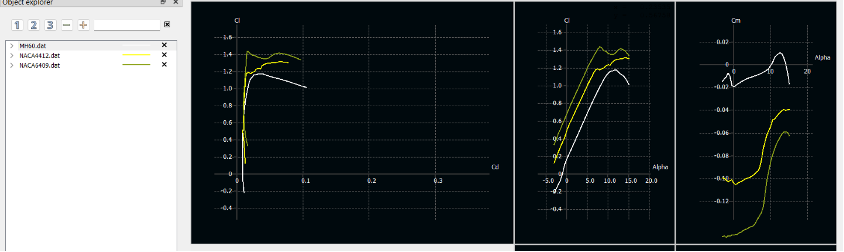
\includegraphics[width=\linewidth]{Figures/main_wing_initial_xlfr5.png}
    \caption[Initial wing XLFR5 analysis results]{The results from running our original three main airfoil choices through XLFR5 with the Reynolds number calculated in \autoref{sec:reynolds}.}
    \label{fig:initial_xlfr5}
\end{figure}

The results from XLFR5 (\autoref{fig:initial_xlfr5}) were imported into the \acrshort{matlab} script shown in \autoref{code:initial_wing_analysis}. From this script, the parameters tabulated in \autoref{tbl:initial_airfoil_analysis} were generated.

\begin{table}[htpb]
    \centering
    \caption[Initial airfoil analysis]{The results of the initial main wing airfoil analysis, where \gls{dC_L-by-dalpha} is the slope of the coefficient versus angle of attack curve, \gls{C_L_max} is the maximum value of the coefficient of lift curve, \gls{C_D_max} is the maximum value of the drag coefficient, and \gls{L-by-D_max} is the maximum value of the lift-drag ratio.}
    \begin{tabular}{cccccc}
        \toprule
        \textbf{Airfoil} & \textbf{\gls{dC_L-by-dalpha}} & \textbf{\gls{C_L_max}} & \textbf{\gls{C_D_max}} & \textbf{\gls{L-by-D_max}} & \textbf{\gls{alpha_stall}} \\
        \midrule
        \acrshort{naca} 4412 & \num{0.1001} & \num{1.3127} & \num{0.0777} & \num{19.3466} & \num{14} \\
        \acrshort{naca} 6409 & \num{0.0990} & \num{1.4378} & \num{0.0962} & \num{17.9252} & \num{8} \\
        \acrshort{mh} 60 & \num{0.1061} & \num{1.1728} & \num{0.1051} & \num{12.0892} & \num{11.5} \\
        \bottomrule
    \end{tabular}
    \label{tbl:initial_airfoil_analysis}
\end{table}

Based on the results in \autoref{tbl:initial_airfoil_analysis}, we chose to move forward with the \acrshort{naca} 4412. It had the best lift-drag ratio and a high stall angle.

\section{Initial Stabilizer Analysis}

Each of the stabilizers have a chord of approximately \qty{15}{\centi\meter}; so, their corresponding Reynolds number is approximately \num{180000} (see \autoref{eq:reynolds}). Plugging the airfoils shown in \autoref{fig:e423_plot} and \autoref{fig:vertical_stabilizer_airfoil_plots} into XFLR5, we obtained the results shown in \autoref{fig:initial_xlfr5_stabilizer-1}.

\begin{figure}[htpb]
    \centering
    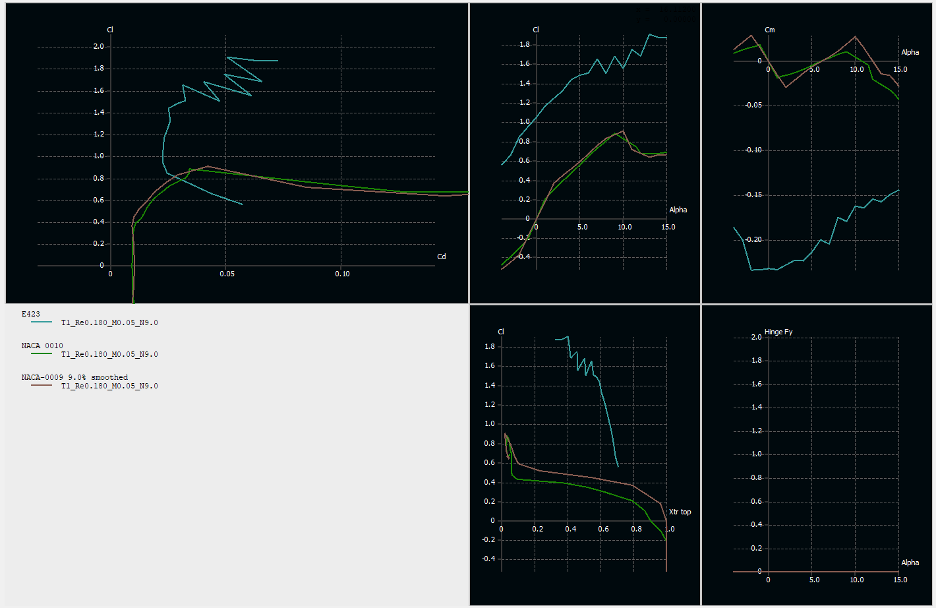
\includegraphics[width=\linewidth]{Figures/stabilizer_initial_xlfr5-1.png}
    \caption[Initial stabilizer XLFR5 analysis results]{The results from running our three stabilizer airfoils through XFLR5.}
    \label{fig:initial_xlfr5_stabilizer-1}
\end{figure}

The \acrshort{naca} 0009 and \acrshort{naca} 0010 converged well, but the \acrshort{e}423 did not. Running the \acrshort{e}432 airfoil again with a higher mach and Reynolds number yielded better results, as shown in \autoref{fig:initial_xlfr5_stabilizer-2}.

\begin{figure}[htpb]
    \centering
    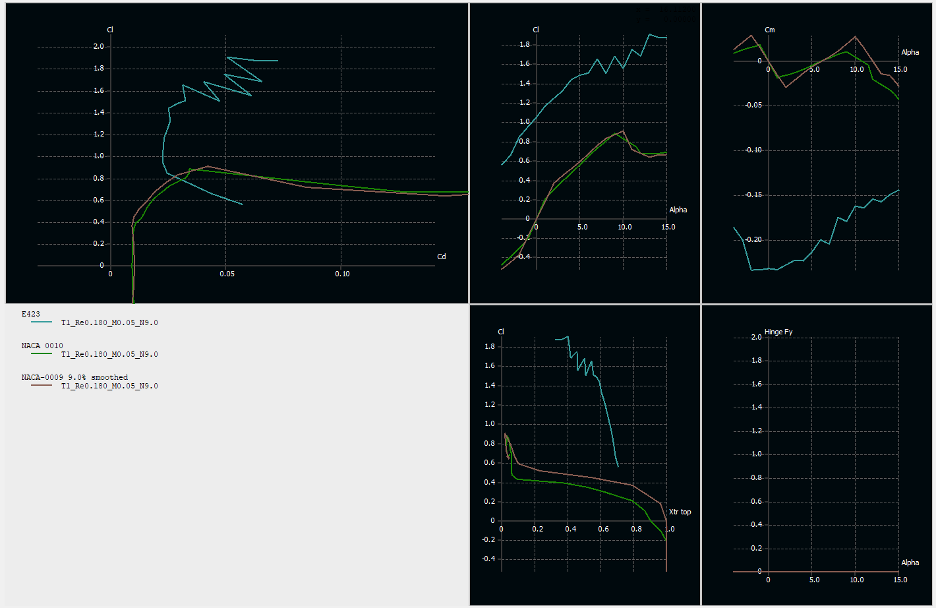
\includegraphics[width=\linewidth]{Figures/stabilizer_initial_xlfr5-1.png}
    \caption[Improved \acrshort{e}423 stabilizer XFLR5 results]{The results from running the \acrshort{e}423 stabilizer in XFLR5 with a higher Reynolds number.}
    \label{fig:initial_xlfr5_stabilizer-2}
\end{figure}

From the data, we began to be concerned that the \acrshort{e}423 would produce too much lift at higher speeds for a horizontal stabilizer, but chose to continue the analysis with the \acrshort{e}423 as our horizontal stabilizer. For the two vertical stabilizers, the data at cruise speed was almost identical, but we decided to move forward with the \acrshort{naca} 0010 because its average pitching moment was closer to zero—and a neutral pitching moment is desirable for a vertical stabilizer.

\section{Reynolds Number Ranges}

At this point in the analysis, we have selected the following airfoils:

\begin{itemize}
    \item Wing: \acrshort{naca} 4412
    \item Horizontal Stabilizer: \acrshort{e}423
    \item Vertical Stabilizer: \acrshort{naca} 0010
\end{itemize}

To further evaluate these choices, we ran XFLR5 analyses for the airfoils at a range of Reynolds number that our \acrshort{uav} would encounter during flight. To get a better sense of the airfoil performance, we chose a Mach number range of \numrange{0.040}{0.080}, which represents a reasonable range of speeds \acrfull{rc} aircraft normally fly at during cruise. The corresponding Reynolds numbers this range produces are shown in \autoref{tbl:reynolds_range}.

\begin{table}[htpb]
    \centering
    \caption[Range of Reynolds numbers]{Range of Reynolds numbers calculated at different Mach numbers \gls{M}.}
    \begin{tabular}{cccccc}
        \toprule
        \textbf{\gls{M}} & \textbf{\gls{Re} (wing)} & \textbf{\gls{Re} (stabilizer)} \\
        \midrule
        \num{0.040} & \num{180000} & \num{135000} \\
        \num{0.053} & \num{240000} & \num{180000} \\
        \num{0.066} & \num{300000} & \num{225000} \\
        \num{0.080} & \num{360000} & \num{270000} \\
    \end{tabular}
    \label{tbl:reynolds_range}
\end{table}

We also calculated Reynolds numbers at ground level, but the results of the ground analysis were nearly identical to the cruise altitude; so, going forward, we will only consider the cruise altitude analysis results.

The results of the XFLR5 analyses with a range of Reynolds numbers are shown in \autoref{fig:final_naca4412}, \autoref{fig:final_e423}, and \autoref{fig:final_naca0010}.

\begin{figure}[htpb]
    \centering
    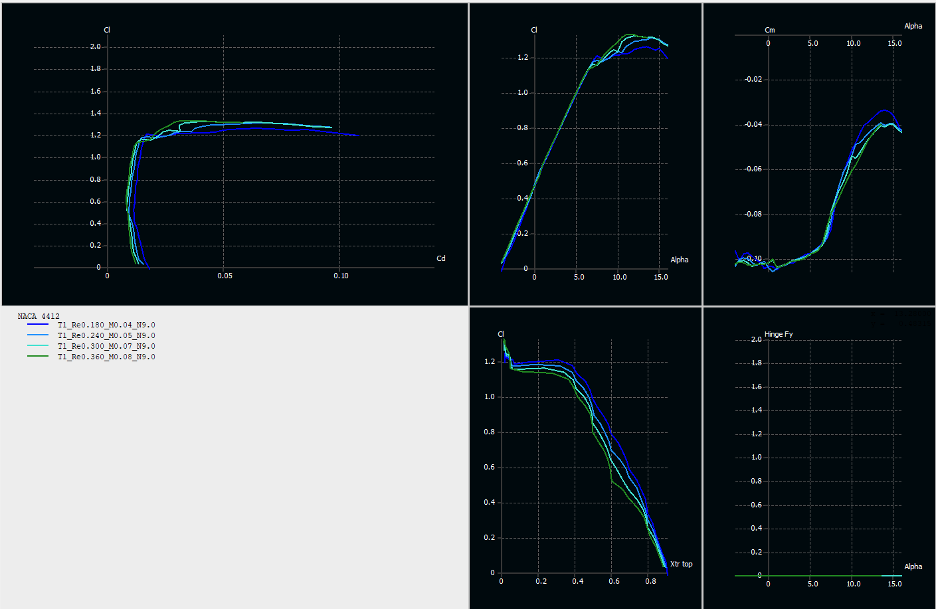
\includegraphics[width=\linewidth]{Figures/final_naca_4412.png}
    \caption[Final XFLR5 analysis of \acrshort{naca} 4412]{The XFLR5 results from running a range of Reynolds numbers on the \acrshort{naca} 4412.}
    \label{fig:final_naca4412}
\end{figure}

\begin{figure}[htpb]
    \centering
    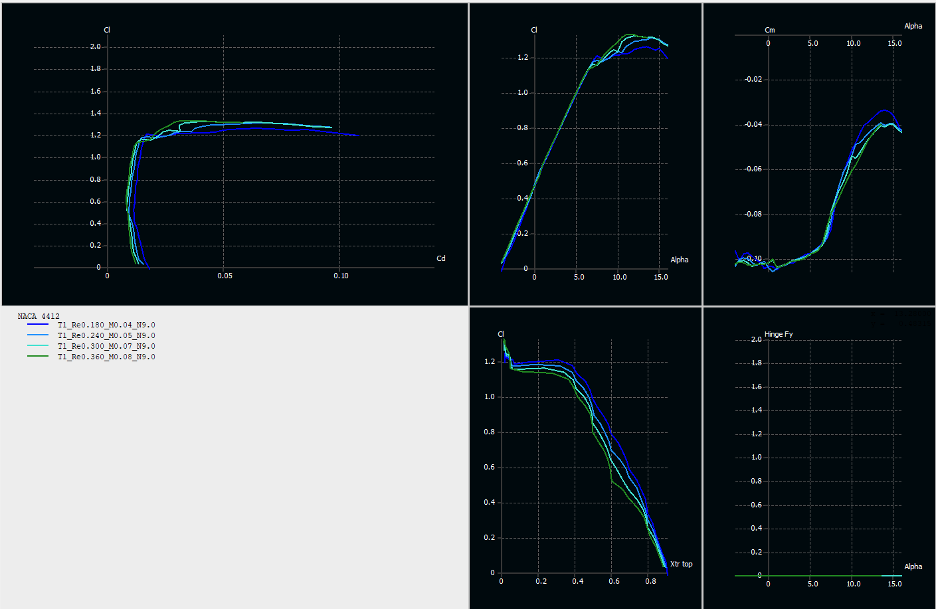
\includegraphics[width=\linewidth]{Figures/final_naca_4412.png}
    \caption[Final XFLR5 analysis of \acrshort{e}423]{The XFLR5 results from running a range of Reynolds numbers on the \acrshort{e}423.}
    \label{fig:final_e423}
\end{figure}

\begin{figure}[htpb]
    \centering
    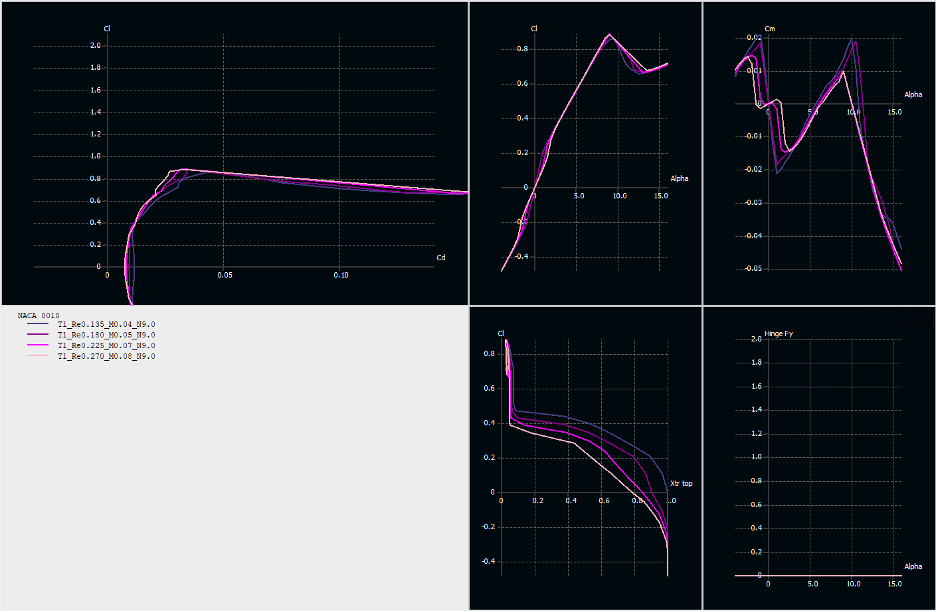
\includegraphics[width=\linewidth]{Figures/final_naca_0010.png}
    \caption[Final XFLR5 analysis of \acrshort{naca} 0010]{The XFLR5 results from running a range of Reynolds numbers on the \acrshort{naca} 0010.}
    \label{fig:final_naca0010}
\end{figure}

\newpage

From these XFLR5 results, we now had a better sense of the airfoils over a range of flight conditions. While we were initially drawn to the \acrshort{e}423 for its high lift-drag ratio, it had widely varying values for its lift coefficient, which may make the \acrshort{uav} unstable if we were to use it for a horizontal stabilizer and fly at high speeds.

Our initial research did point us towards using a symmetric airfoil for the horizontal stabilizer, but we wanted to experiment with a cambered airfoil. Based on these discouraging XFLR5 results, we decided to fall back to the \acrshort{naca} 0010 as both the horizontal and vertical stabilizer. The \acrshort{naca} 4412 continued to seem like a good option for a main wing airfoil.
